\documentclass[tikz,border=8pt]{standalone}
\definecolor{wall}{HTML}{DCEBF7}
\definecolor{wallline}{HTML}{C5DAEC}
\definecolor{floor}{HTML}{D8B98F}
\definecolor{floordark}{HTML}{B8955F}
\definecolor{wood}{HTML}{9C6B3E}
\definecolor{wooddark}{HTML}{7A5030}
\definecolor{bedsheet}{HTML}{7FB3E6}
\definecolor{beddark}{HTML}{4F86BF}
\definecolor{pillow}{HTML}{FFFFFF}
\definecolor{blanket}{HTML}{F2C14E}
\definecolor{skin}{HTML}{F6D3B4}
\definecolor{boyhair}{HTML}{4A3325}
\definecolor{boyshirt}{HTML}{E9553E}
\definecolor{boypants}{HTML}{3B5B8C}
\definecolor{vr}{HTML}{2E2E36}
\definecolor{vrlight}{HTML}{6EE7F9}
\definecolor{momhair}{HTML}{6B4A2E}
\definecolor{momdress}{HTML}{6DA875}
\definecolor{momdressdark}{HTML}{4E8256}
\definecolor{door}{HTML}{B98457}
\definecolor{hall}{HTML}{F4E6C9}
\definecolor{gaze}{HTML}{E0742A}
\definecolor{book1}{HTML}{E76F51}
\definecolor{book2}{HTML}{2A9D8F}
\definecolor{book3}{HTML}{E9C46A}
\definecolor{book4}{HTML}{8E6BA8}
\begin{document}
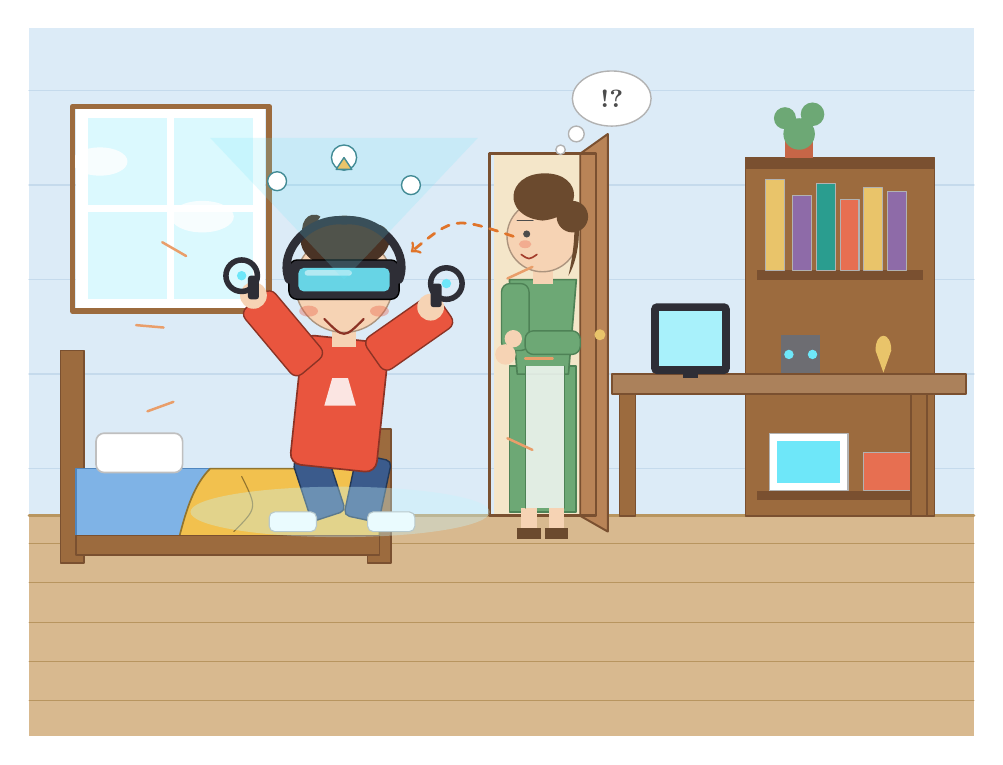
\begin{tikzpicture}[x=1cm,y=1cm,line join=round,line cap=round]
  % room 12 x 9
  \fill[wall] (0,0) rectangle (12,9);
  \foreach \y in {3.4,4.6,5.8,7.0,8.2}{\draw[wallline,line width=0.5pt] (0,\y) -- (12,\y);}
  \fill[floor] (0,0) rectangle (12,2.8);
  \foreach \y in {0.45,0.95,1.45,1.95,2.45}{\draw[floordark,line width=0.4pt] (0,\y) -- (12,\y);}
  \draw[floordark,line width=1pt] (0,2.8) -- (12,2.8);

  % --- window (top-left) ---
  \fill[white] (0.6,5.4) rectangle (3.0,8.0);
  \fill[vrlight!25!white] (0.75,5.55) rectangle (2.85,7.85);
  \fill[white,opacity=0.8] (0.9,7.3) ellipse (0.35 and 0.18);
  \fill[white,opacity=0.8] (2.2,6.6) ellipse (0.4 and 0.2);
  \draw[white,line width=2.5pt] (1.8,5.55) -- (1.8,7.85) (0.75,6.7) -- (2.85,6.7);
  \draw[wood,line width=2pt] (0.55,5.4) rectangle (3.05,8.0);

  % --- bed (left) ---
  \fill[wood,draw=wooddark,line width=0.6pt] (0.4,2.2) rectangle (0.7,4.9);
  \fill[wood,draw=wooddark,line width=0.6pt] (4.3,2.2) rectangle (4.6,3.9);
  \fill[bedsheet,draw=beddark,line width=0.6pt] (0.6,2.5) rectangle (4.45,3.4);
  \fill[blanket,draw=blanket!60!black,line width=0.6pt] (1.9,2.5) -- (4.45,2.5) -- (4.45,3.4) -- (2.3,3.4) .. controls (2.1,3.2) and (2.0,2.9) .. (1.9,2.5) -- cycle;
  \draw[blanket!60!black,line width=0.4pt] (2.6,2.6) .. controls (2.9,2.9) .. (2.7,3.3);
  \fill[pillow,draw=black!25,line width=0.6pt,rounded corners=3pt] (0.85,3.35) rectangle (1.95,3.85);
  \fill[wood,draw=wooddark,line width=0.6pt] (0.6,2.3) rectangle (4.45,2.55);
  % plush on the bed
  \fill[boyshirt!40!white] (3.6,3.5) circle (0.22);
  \fill[boyshirt!40!white] (3.45,3.7) circle (0.09) (3.75,3.7) circle (0.09);
  \fill[black!70] (3.53,3.53) circle (0.03) (3.67,3.53) circle (0.03);

  % --- bookshelf & desk (right) ---
  \fill[wood,draw=wooddark,line width=0.6pt] (9.1,2.8) rectangle (11.5,7.35);
  \foreach \y in {3.0,4.4,5.8}{\fill[wooddark] (9.25,\y) rectangle (11.35,\y+0.12);}
  \fill[wooddark] (9.1,7.2) rectangle (11.5,7.35);
  % small plant on top of the shelf
  \fill[book1!70!wooddark] (9.6,7.35) rectangle (9.95,7.65);
  \fill[momdress] (9.78,7.65) circle (0.2) (9.6,7.85) circle (0.14) (9.95,7.9) circle (0.15);
  \foreach \x/\c/\h in {9.35/book3/1.2,9.7/book4/1.0,10.0/book2/1.15,10.3/book1/0.95,10.6/book3/1.1,10.9/book4/1.05}{
    \fill[\c,draw=black!30,line width=0.4pt] (\x,5.92) rectangle (\x+0.24,5.92+\h-0.05);
  }
  % robot toy + trophy
  \fill[vr!70!white] (9.55,4.52) rectangle (10.05,5.1);
  \fill[vrlight] (9.65,4.85) circle (0.06) (9.95,4.85) circle (0.06);
  \fill[book3] (10.7,4.52) rectangle (11.0,4.62);
  \fill[book3] (10.85,4.62) -- (10.75,4.9) .. controls (10.75,5.15) and (10.95,5.15) .. (10.95,4.9) -- cycle;
  % game console box on the bottom shelf
  \fill[white,draw=black!30,line width=0.4pt] (9.4,3.12) rectangle (10.4,3.85);
  \fill[vrlight] (9.5,3.22) rectangle (10.3,3.75);
  \fill[book1,draw=black!30,line width=0.4pt] (10.6,3.12) rectangle (11.2,3.6);

  % desk with monitor on the far right side
  \fill[wood,draw=wooddark,line width=0.6pt] (11.2,2.8) rectangle (11.4,4.4);
  \fill[wood!85!white,draw=wooddark,line width=0.6pt] (7.4,4.35) rectangle (11.9,4.6);
  \fill[wood,draw=wooddark,line width=0.6pt] (7.5,2.8) rectangle (7.7,4.35);
  \fill[vr,rounded corners=2pt] (7.9,4.6) rectangle (8.9,5.5);
  \fill[vrlight!60!white] (8.0,4.7) rectangle (8.8,5.4);
  \fill[vr] (8.3,4.55) rectangle (8.5,4.65);

  % --- door + mother (right edge) ---
  \fill[hall] (5.9,2.8) rectangle (7.2,7.4);
  \fill[door,draw=wooddark,line width=0.7pt] (7.0,2.8) -- (7.35,2.6) -- (7.35,7.65) -- (7.0,7.4) -- cycle;
  \draw[wooddark,line width=1pt] (5.85,2.8) rectangle (7.2,7.4);
  \fill[book3] (7.25,5.1) circle (0.07);
  % mother, standing in the doorway, facing the boy (left)
  \fill[momdress,draw=momdressdark,line width=0.6pt] (6.1,2.85) rectangle (6.95,4.7);
  \fill[momdress,draw=momdressdark,line width=0.6pt] (6.2,4.6) -- (6.85,4.6) -- (6.95,5.8) -- (6.1,5.8) -- cycle;
  \fill[skin] (6.25,2.6) rectangle (6.45,2.9);
  \fill[skin] (6.6,2.6) rectangle (6.8,2.9);
  \fill[momhair] (6.2,2.5) rectangle (6.5,2.65);
  \fill[momhair] (6.55,2.5) rectangle (6.85,2.65);
  % arm holding the door frame / arms folded
  \fill[momdress,draw=momdressdark,line width=0.5pt,rounded corners=3pt] (6.0,4.9) rectangle (6.35,5.75);
  \fill[momdress,draw=momdressdark,line width=0.5pt,rounded corners=3pt] (6.3,4.85) rectangle (7.0,5.15);
  \fill[skin] (6.05,4.85) circle (0.13);
  \fill[skin] (6.15,5.05) circle (0.11);
  % apron
  \fill[white,opacity=0.8] (6.3,2.9) rectangle (6.8,4.7);
  \draw[momdressdark,line width=0.4pt] (6.3,4.7) -- (6.3,2.9) (6.8,4.7) -- (6.8,2.9);
  % head (looking left)
  \fill[skin] (6.4,5.75) rectangle (6.65,5.95);
  \fill[skin,draw=skin!70!black,line width=0.5pt] (6.52,6.35) circle (0.45);
  \fill[momhair] (6.52,6.55) .. controls (6.0,6.6) and (6.05,7.15) .. (6.55,7.15) .. controls (7.05,7.15) and (7.05,6.6) .. (6.52,6.55) -- cycle;
  \fill[momhair] (6.85,6.9) .. controls (7.05,6.6) and (7.0,6.1) .. (6.85,5.85) .. controls (6.95,6.3) and (6.95,6.6) .. (6.85,6.9) -- cycle;
  \fill[momhair] (6.9,6.6) circle (0.2);
  \fill[black!70] (6.32,6.38) circle (0.045);
  \draw[black!70,line width=0.5pt] (6.2,6.55) -- (6.4,6.55);
  \draw[boyshirt!70!black,line width=0.6pt] (6.25,6.12) .. controls (6.35,6.05) .. (6.45,6.12);
  \fill[boyshirt,opacity=0.3] (6.3,6.25) ellipse (0.08 and 0.05);
  % thought bubble ("!?")
  \fill[white,draw=black!30,line width=0.5pt] (6.75,7.45) circle (0.06);
  \fill[white,draw=black!30,line width=0.5pt] (6.95,7.65) circle (0.1);
  \fill[white,draw=black!30,line width=0.5pt] (7.4,8.1) ellipse (0.5 and 0.35);
  \node[font=\bfseries\small,text=black!70] at (7.4,8.1) {!?};

  % --- boy in the centre, playing VR ---
  % motion lines
  \foreach \a in {150,175,200}{\draw[gaze!70!white,line width=0.9pt] (3.9,5.0) ++(\a:2.2) -- ++(\a:0.35);}
  \foreach \a in {-25,0,25}{\draw[gaze!70!white,line width=0.9pt] (3.9,4.8) ++(\a:2.4) -- ++(\a:0.35);}
  % legs (dynamic stance)
  \fill[boypants,draw=boypants!60!black,line width=0.5pt,rounded corners=2pt,rotate around={18:(3.55,3.5)}] (3.35,2.75) rectangle (3.8,3.55);
  \fill[boypants,draw=boypants!60!black,line width=0.5pt,rounded corners=2pt,rotate around={-12:(4.35,3.5)}] (4.15,2.75) rectangle (4.6,3.55);
  \fill[white,draw=black!30,line width=0.4pt,rounded corners=2pt] (3.05,2.6) rectangle (3.65,2.85);
  \fill[white,draw=black!30,line width=0.4pt,rounded corners=2pt] (4.3,2.6) rectangle (4.9,2.85);
  % torso
  \fill[boyshirt,draw=boyshirt!60!black,line width=0.6pt,rounded corners=4pt,rotate around={-6:(3.95,4.3)}] (3.4,3.4) rectangle (4.5,5.05);
  \fill[white,opacity=0.85] (3.75,4.2) -- (4.15,4.2) -- (4.05,4.55) -- (3.85,4.55) -- cycle;
  % arms raised, holding controllers
  \fill[boyshirt,draw=boyshirt!60!black,line width=0.5pt,rounded corners=3pt,rotate around={40:(3.45,4.85)}] (3.2,4.65) rectangle (3.7,5.75);
  \fill[boyshirt,draw=boyshirt!60!black,line width=0.5pt,rounded corners=3pt,rotate around={-55:(4.5,4.9)}] (4.25,4.75) rectangle (4.75,5.85);
  \fill[skin] (2.85,5.6) circle (0.17);
  \fill[skin] (5.1,5.45) circle (0.17);
  % controllers (rings)
  \draw[vr,line width=2pt] (2.7,5.85) circle (0.2);
  \fill[vr,rounded corners=1pt] (2.78,5.55) rectangle (2.92,5.85);
  \draw[vr,line width=2pt] (5.3,5.75) circle (0.2);
  \fill[vr,rounded corners=1pt] (5.1,5.45) rectangle (5.24,5.75);
  \fill[vrlight] (2.7,5.85) circle (0.06) (5.3,5.75) circle (0.06);
  % neck + head
  \fill[skin] (3.85,4.95) rectangle (4.15,5.25);
  \fill[skin,draw=skin!70!black,line width=0.5pt] (4.0,5.75) circle (0.62);
  \fill[boyhair] (4.0,5.95) .. controls (3.3,5.95) and (3.35,6.55) .. (3.7,6.5) .. controls (3.8,6.65) and (4.2,6.65) .. (4.35,6.5) .. controls (4.7,6.55) and (4.7,5.95) .. (4.0,5.95) -- cycle;
  \fill[boyhair] (3.5,6.3) .. controls (3.4,6.5) and (3.55,6.7) .. (3.7,6.6) -- cycle;
  % VR headset
  \fill[vr,draw=black,line width=0.5pt,rounded corners=3pt] (3.3,5.55) rectangle (4.7,6.05);
  \fill[vrlight,opacity=0.9,rounded corners=2pt] (3.42,5.65) rectangle (4.58,5.95);
  \fill[white,opacity=0.5,rounded corners=1pt] (3.5,5.85) rectangle (4.1,5.92);
  \draw[vr,line width=3pt] (3.3,5.8) .. controls (3.15,6.2) and (3.6,6.6) .. (4.0,6.55) .. controls (4.4,6.6) and (4.85,6.2) .. (4.7,5.8);
  % big smile below the headset
  \draw[boyshirt!60!black,line width=0.8pt] (3.75,5.3) .. controls (4.0,5.05) .. (4.25,5.3);
  \fill[boyshirt,opacity=0.35] (3.55,5.4) ellipse (0.12 and 0.07) (4.45,5.4) ellipse (0.12 and 0.07);
  % rug under the boy
  \fill[vrlight!40!white,opacity=0.35] (3.95,2.85) ellipse (1.9 and 0.32);

  % --- gaze relationship: mother -> boy (boy can't see her) ---
  \draw[gaze,dashed,line width=1pt,->] (6.15,6.35) .. controls (5.4,6.6) .. (4.85,6.15);
  % headset "view" cone: the boy sees the virtual world, not the room
  \fill[vrlight,opacity=0.18] (4.0,5.8) -- (2.3,7.6) -- (5.7,7.6) -- cycle;
  \fill[white,draw=vrlight!60!black,line width=0.5pt] (3.15,7.05) circle (0.12);
  \fill[white,draw=vrlight!60!black,line width=0.5pt] (4.0,7.35) circle (0.16);
  \fill[white,draw=vrlight!60!black,line width=0.5pt] (4.85,7.0) circle (0.12);
  \fill[book3,draw=vrlight!60!black,line width=0.5pt] (4.0,7.35) -- (3.9,7.2) -- (4.1,7.2) -- cycle;
\end{tikzpicture}
\end{document}
